\section{Dataset Description}
\label{sec:ds_desc}
The dataset selected to address our goal is the ``Stellar Classification Dataset - SDSS17'', available on Kaggle~\cite{kaggle}.

This dataset contains 100,000 observations of space taken by the \textit{SDSS (Sloan Digital Sky Survey)}. Every observation is described by 17 \textit{feature} columns and 1 \textit{class} column which identifies it to be either a star, galaxy or quasar.

 \begin{itemize}
    \item \texttt{obj\_ID}: Unique identifier for each astronomical object, used by the CAS.
    \item \texttt{alpha}: Right ascension angle \\(J2000 epoch).
    \item \texttt{delta}: Declination angle \\(J2000 epoch).
    \item \texttt{u}: Ultraviolet filter in the photometric system.
    \item \texttt{g}: Green filter in the photometric system.
    \item \texttt{r}: Red filter in the photometric system.
    \item \texttt{i}: Near-infrared filter in the photometric system.
    \item \texttt{z}: Infrared  filter in the photometric system.
    \item \texttt{run\_ID}: Run number, which identifies the specific scan.
    \item \texttt{rerun\_ID}: Rerun number, which specifies how the image was processed.
    \item \texttt{cam\_col}: Camera column, which\\indicates the scanline within the run.
    \item \texttt{field\_ID}: Field number, which identifies each field.
    \item \texttt{spec\_obj\_ID}: Unique identifier for optical spectroscopic objects. This means that 2 different observations with the same value of this ID must share the output class.
    \item \texttt{class}: Object class (galaxy, star or quasar).
    \item \texttt{redshift}: Redshift value, based on the increase in wavelength.
    \item \texttt{plate}: Identifier for each SDSS plate.
    \item \texttt{MJD}: Modified Julian Date, indicating when a piece of SDSS data was taken.
    \item \texttt{fiber\_ID}: Specifies the fiber that pointed the light at the focal plane in each observation.
\end{itemize}

\bigskip

\subsection{Class Distribution}
% Put Image
\begin{figure}[H]
    \centering
    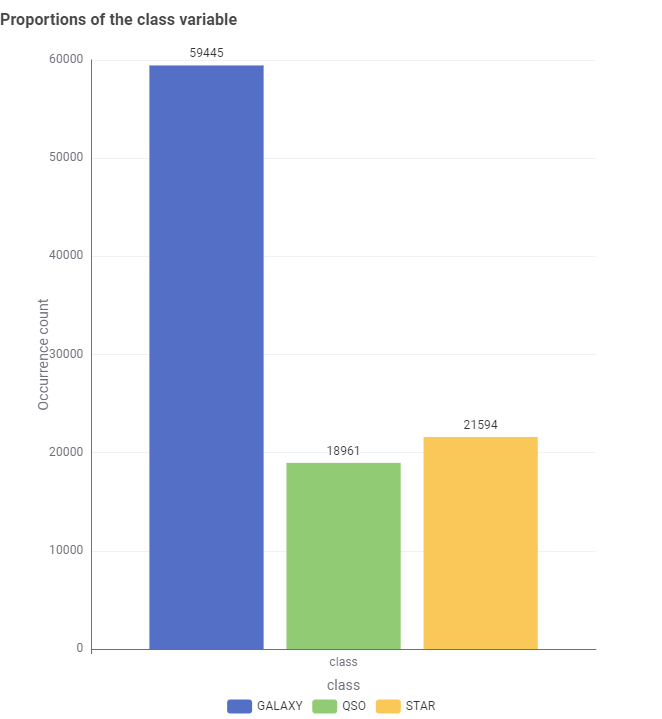
\includegraphics[width=1\columnwidth]{images/Bar Chart.png}
    \caption{Proportions of the unbalanced dataset.}
    \label{fig:classes}
\end{figure}
%Following, there are the number of observations for the class variable:
%\begin{itemize}
%    \item Galaxies: 59,445.
%    \item Quasars: 18,961.
%    \item Stars: 21,594.
%\end{itemize}

As we can see from Fig.~\ref{fig:classes}, quasars appeared less frequently compared to galaxies and stars, aligning with the expectation that quasars are rarer and further celestial objects.\\The dataset is \textit{unbalanced} with respect to the target variable. This needs to be taken into account and addressed, and it will be further analyzed.
%\vspace{0.5cm}